\documentclass[a4paper]{article}
\def\DOCTITLE{CSC3424 Bio Algorithms}
% Set document attributes
\title{\DOCTITLE}

\usepackage{fullpage}
\usepackage{scrextend}
\usepackage{titlesec}
\usepackage{fancyhdr}
\usepackage{amsmath}
\usepackage{amssymb}
\usepackage[section]{placeins}
\usepackage{booktabs}
\usepackage{hyperref}
\usepackage{tikz}
\usepackage{graphicx}
\usepackage{minted}
\usepackage{subcaption}

% Setup headers and footers
\pagestyle{fancy}
\lhead{}
\chead{\DOCTITLE}
\rhead{}
\rfoot{}
\cfoot{\thepage}
\lfoot{}

% New page for each section
\newcommand{\sectionbreak}{\clearpage}

% Set header and footer sizes
\renewcommand{\headrulewidth}{0.4pt}
\renewcommand{\footrulewidth}{0.4pt}
\setlength{\headheight}{15.2pt}
\setlength{\headsep}{15.2pt}

\setlength{\parskip}{5pt plus 1pt minus 1pt}
\setlength{\parindent}{0pt}

% Newline after paragraph
\newcommand{\Para}[1]{\paragraph{#1}\mbox{}}

% Stuff used in cryptography notes
\newcommand{\Forall}{\;\forall\;}
\newcommand{\Mod}{\: mod \:}

% Stuff used in distributed systems notes
\newcommand{\happenbefore}{\rightarrow}
\newcommand{\orderbefore}{\Rightarrow}
\newcommand{\clockcond}{\leadsto}
\newcommand{\RArrow}{$\rightarrow$}

\def\checkmark{\tikz\fill[scale=0.4](0,.35) -- (.25,0) -- (1,.7) -- (.25,.15) -- cycle;}


\begin{document}

\tableofcontents

\section{Cell and Molecular biology}

\subsection{The Cell}

\begin{itemize}
  \item Minimal unit of life
  \item Cell is a system of many components enclosed in a series of membranes
  \item Small organisms such as fungi and bacteria are unicellular
  \item Plants and animals are generally multicellular
\end{itemize}

\subsubsection{Prokaryotes}

\begin{itemize}
  \item All prokaryotes are single cell
  \item Smaller than eukaryotic cells \\
        ($< 1 \mu \mathrm{m}$ in diameter)
  \item Simple structure \\
        No inner cellular membranes
  \item Very adaptable to environment \\
        Found in almost every habitat
  \item Approximately $5x10^{30}$ prokaryotic cells in the world
  \item Essential for healthy life
\end{itemize}

\Para{Prokaryotic cell}

\begin{itemize}
  \item Less complex than eukaryotic cells
  \item Contain no organelles
  \item Believed to represent the earliest life on earth and that eukaryotic
        cells evolved from prokaryotic cells
\end{itemize}

\begin{figure}[h!]
  \centering
  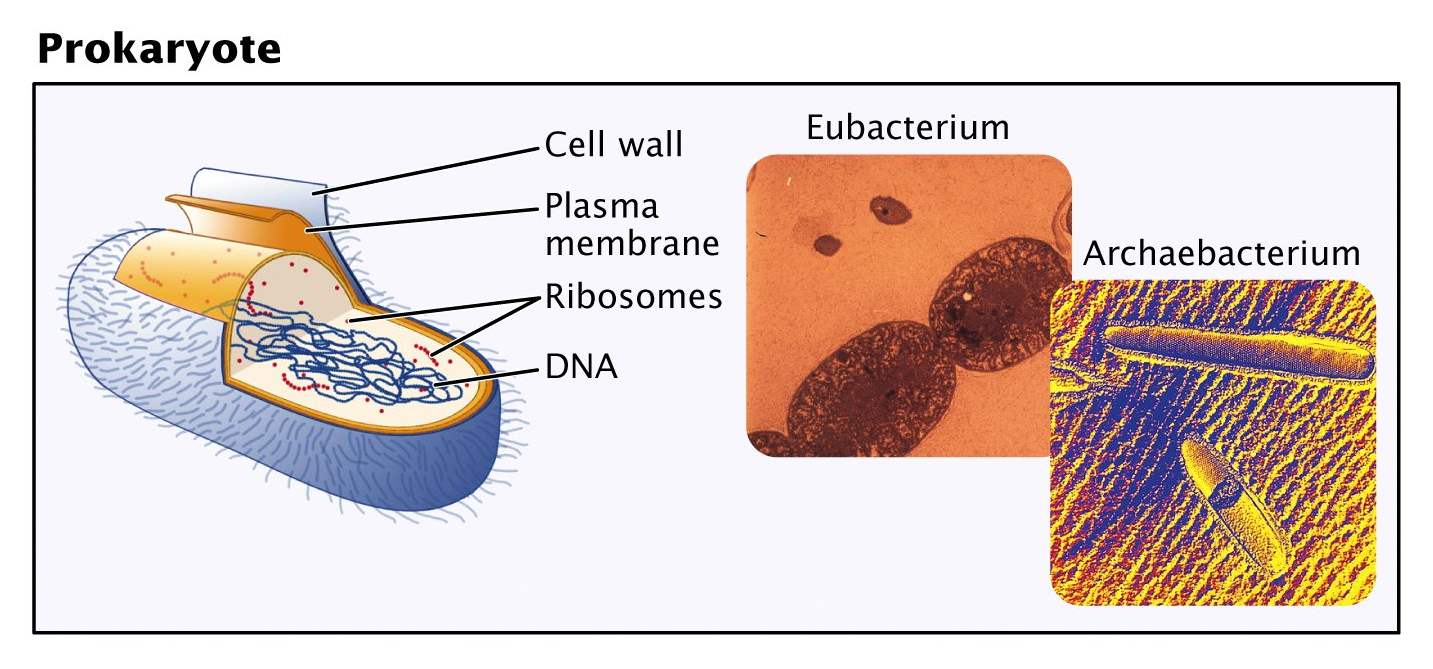
\includegraphics[width=0.7\textwidth]{graphics/prokaryotic_cell.eps}
  \caption{Prokaryotic cell structure}
  \label{fig:prokaryotic_cell}
\end{figure}
\FloatBarrier

\Para{Types of prokaryotes}

Types descend from common ancestor.

\begin{description}
  \item[Eubacteria] \hfill \\
    Common bacteria that affects life daily
  \item[Archaea] \hfill \\
    Tend to exist in extreme habitats (high pressure, temperature, pH)
\end{description}

\subsubsection{Eukaryotes}

\begin{itemize}
  \item More structurally and biochemically complex than prokaryotes
  \item Evolutionarily more recent
  \item Believed to have evolved through endosymbiosis
\end{itemize}

\begin{figure}[h!]
  \centering
  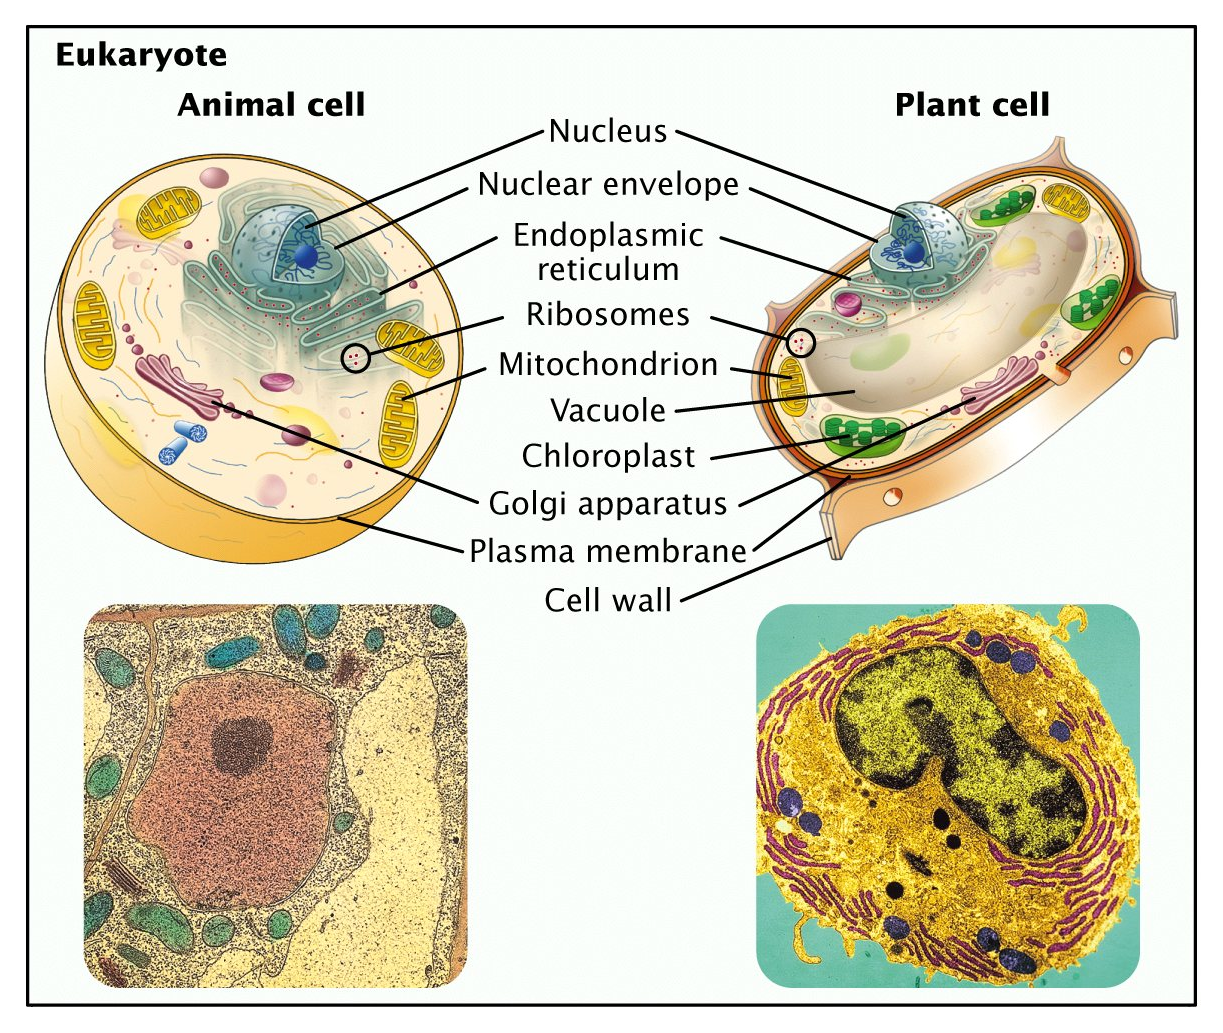
\includegraphics[width=0.7\textwidth]{graphics/eukaryotic_cell.eps}
  \caption{Eukaryotic cell structure}
  \label{fig:eukaryotic_cell}
\end{figure}
\FloatBarrier

\Para{Endosymbiosis}

\begin{itemize}
  \item An ancestral cell engulfed a smaller microbe which continued to survive
        inside it
  \item Both host and prey adapt to new environment and become mutually
        interdependent
\end{itemize}

\subsubsection{Cell functions}

Functions of cells provided by organelle.

\begin{description}
  \item[Nucleus] \hfill \\
    Regulate DNA carrying/replication
  \item[Endoplasmic reticulum] \hfill \\
    System of folded membranes used for transport
  \item[Ribosomes] \hfill \\
    Used to produce proteins
  \item[Mitochondria] \hfill \\
    Provide energy through cellular respiration
  \item[Vacuole] \hfill \\
    Used for storage
  \item[Chloroplasts] \hfill \\
    Used to convert light energy into chemical energy for cell
  \item[Golgi Apparatus] \hfill \\
    Packages and transports proteins
\end{description}

\begin{table}[h!]
  \centering
  \begin{tabular}{@{}lll@{}}
    \toprule
                                & Prokaryotic cells                             & Eukaryotic cells \\
    \midrule
    Nucleus                     & Absent                                        & Present \\
    Cell diameter               & $1-10 \mu \mathrm{m}$                         & $10-100 \mu \mathrm{m}$ \\
    Genome                      & One circular module                           & Multiple linear modules \\
    DNA                         & Not complexed in eubacteria, some in archaea  & Complexed with histomes\\
    DNA quantity                & Small                                         & Large \\
    Membrane-bounded organelles & Absent                                        & Present \\
    Cytoskeleton                & Absent                                        & Present \\
    \bottomrule
  \end{tabular}
  \caption{Comparison of cell types}
  \label{tab:cell_comparison}
\end{table}
\FloatBarrier

\subsubsection{Phenotype from Genotype}

\begin{itemize}
  \item Characteristics of an organism (phenotype) are determined by the
        structure and function of its cells (genotype)
\end{itemize}

\subsection{DNA and genes}

\begin{figure}[h!]
  \centering
  \includegraphics[width=0.2\textwidth]{out/dogma_molecular_biology.eps}
  \caption{Central dogma of molecular biology}
  \label{fig:eukaryotic_cell}
\end{figure}
\FloatBarrier

\subsubsection{Structure of DNA}

\begin{itemize}
  \item Base \\
    Bases bind (A-T, C-G) by Hydrogen bonds
    \begin{itemize}
      \item Pyrimidines
        \begin{itemize}
          \item Cytosine
          \item Thymine
        \end{itemize}
      \item Purines
        \begin{itemize}
          \item Guanine
          \item Adenine
        \end{itemize}
    \end{itemize}
  \item Backbone
    \begin{itemize}
      \item Phosphate \\
        Binds ribose sugar
      \item Ribose sugar \\
        Binds phosphate to base
    \end{itemize}
\end{itemize}

\Para{DNA directionality}

\begin{figure}[h!]
  \centering
  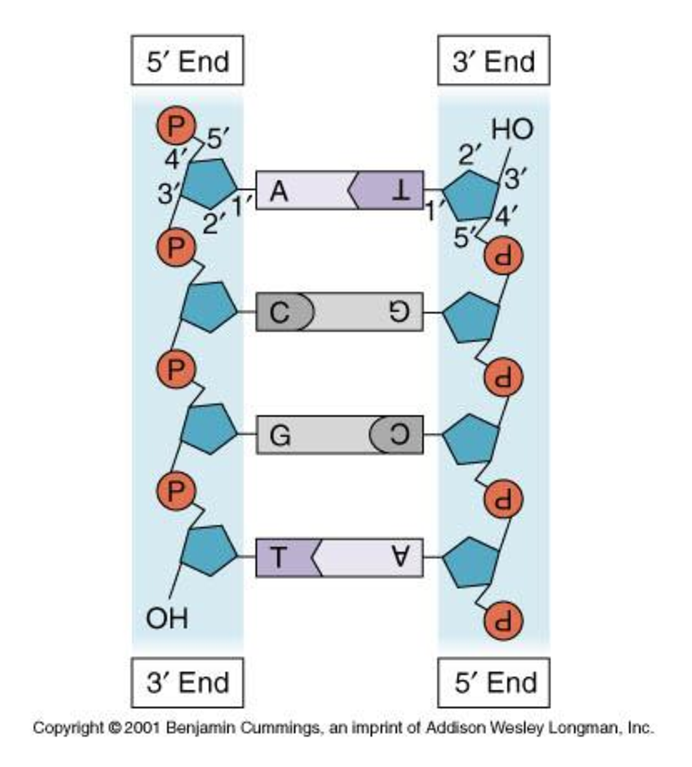
\includegraphics[width=0.4\textwidth]{graphics/dna_directionality.eps}
  \caption{DNA directionality}
  \label{fig:eukaryotic_cell}
\end{figure}
\FloatBarrier

\subsubsection{DNA replication}

\begin{itemize}
  \item Replication is essential for organisms to reproduce
  \item Without replication, cell division could not occur
  \item Replication must be high fidelity but have potential for error (to
        enable evolution)
\end{itemize}

\Para{C-value paradox}

The C-value is the size of an organisms genome (defined as the amount of DNA in
pico grams in a haploid cell).

C-values not reflective of complexity, i.e. no relation between C-value and
number of genes.

\subsubsection{Genome structure}

\Para{Prokaryotic}

\begin{itemize}
  \item Generally small ($<10 \mathrm{M}$ bases)
  \item Single, circular chromosome
  \item Can have plasmids \\
        Disposable genetic elements that often carry genes for antibiotic
        resistance or toxicity
  \item Information dense \\
        Little or no space between genes, genes often overlap
  \item Genes are present in single, uninterrupted units
  \item Multiple genes may be present in single, uninterrupted units
\end{itemize}

\Para{Eukaryotic}

\begin{itemize}
  \item Usually larger than prokaryotic genomes
  \item Multiple, linear chromosomes
  \item Tend to be more information sparse \\
        Large gaps between genes
  \item Genes interrupted by non-coding sequence
    \begin{description}
      \item[Exons] coding
      \item[Introns] non-coding
    \end{description}
\end{itemize}

\subsubsection{DNA packaging}

Nuclear DNA is packaged as chromatin, a structure of DNA, RNA and protein.

Purpose of chromatin:
\begin{itemize}
  \item Packages DNA into a more compact structure
  \item Reinforces macromolecule to allow mitosis
  \item Prevents DNA damage
  \item Regulates gene expression and DNA replication
\end{itemize}

\begin{figure}[h!]
  \centering
  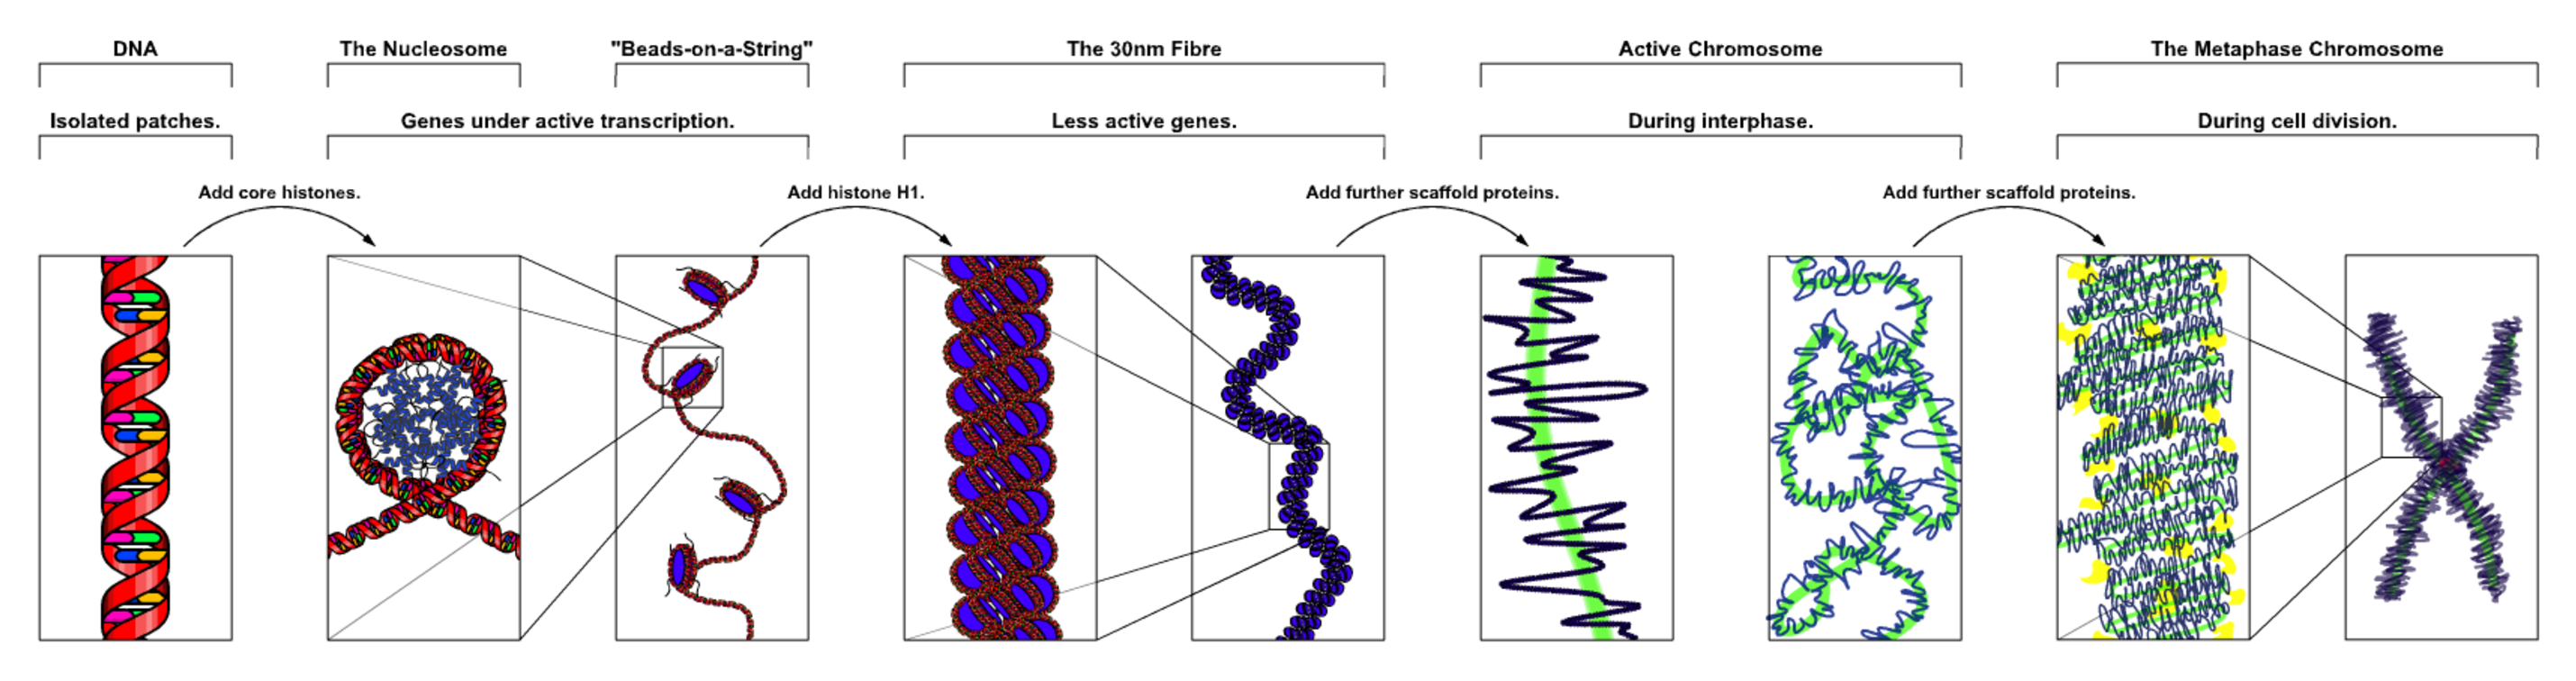
\includegraphics[width=\textwidth]{graphics/chromatin_structures.eps}
  \caption{Chromatin structure}
  \label{fig:chromatin_structures}
\end{figure}
\FloatBarrier

\subsubsection{Manipulating genomes}

\begin{itemize}
  \item Genetic engineering gives multiple techniques for editing the genome of
        an organism
  \item Simplest example is artificial selection to obtain desired traits
  \item Synthetic biology apples engineering principles to biology
\end{itemize}

\subsubsection{Gene structure}

\begin{itemize}
  \item Genes encode functional RNA modules
  \item A gene is a functional part of a chromosome
  \item Every cell contains the same set of genes
\end{itemize}

\subsection{Transcription}

Process of turning information stored in DNA into RNA.

\begin{description}
  \item[Non-template (coding) strand] \hfill \\
    Contains same base sequence as RNA crated
  \item[Template (non-coding) strand] \hfill \\
    Contains anti-codons of RNA
  \item[Promoter] \hfill \\
    Denotes start of RNA coding region
  \item[Coding region] \hfill \\
    RNA coding
  \item[Terminator] \hfill \\
    DNA coding denoting the end of the coding region
\end{description}

\begin{figure}[h!]
  \centering
  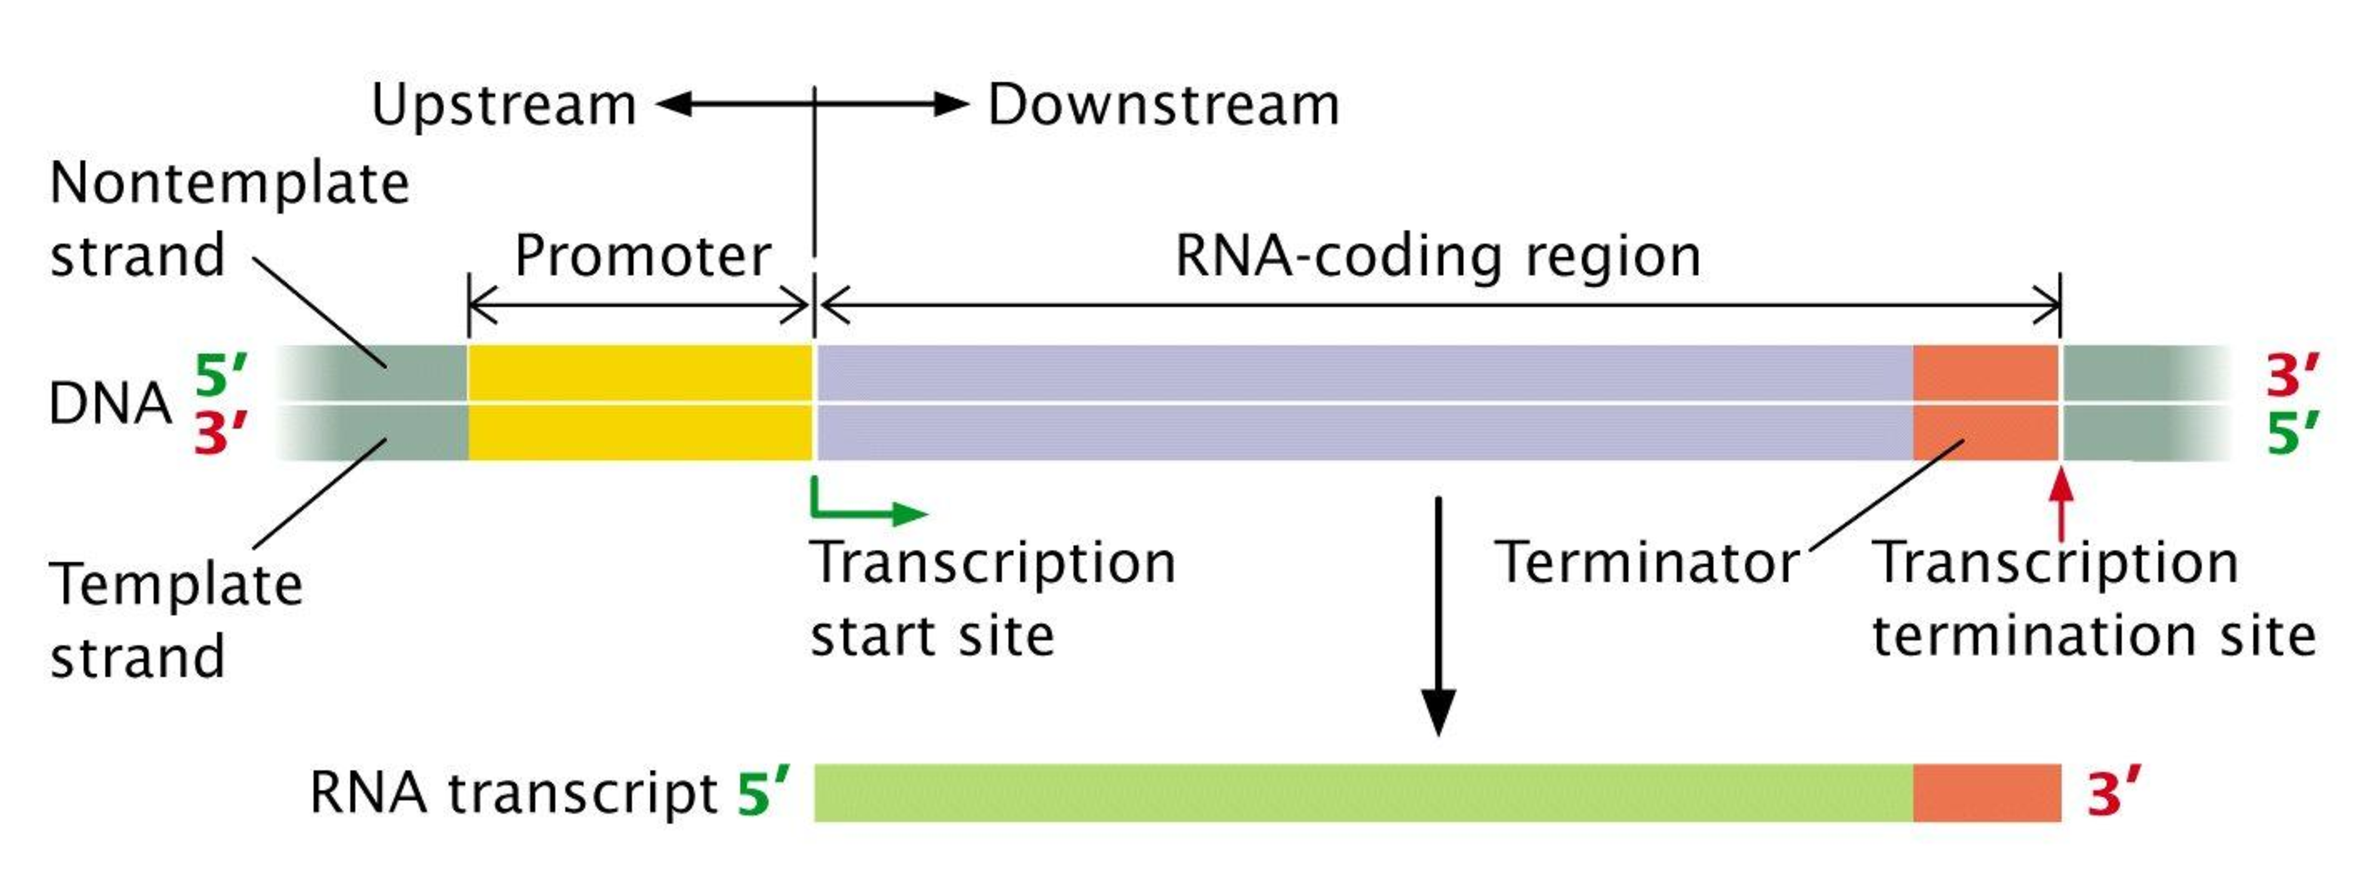
\includegraphics[width=0.8\textwidth]{graphics/dna-rna_transcription.eps}
  \caption{DNA directionality}
  \label{fig:dna-rna_transcription}
\end{figure}
\FloatBarrier

\begin{itemize}
  \item The base Thymine (T) in DNA is replaced with Uracil (U) in RNA
  \item Transcription occurs $5^{\prime}$ to $3^{\prime}$
  \item RNA polymerase is the enzyme responsible for transcription
  \item Transcription in eukaryotes is more complex
\end{itemize}

\subsubsection{Transcript processing}

Primary transcript must be processed into a mature message.

\begin{itemize}
  \item Addition of $5^{\prime}$ cap
    \begin{itemize}
      \item 7-methlyguanosine
      \item Involved in ribosome binding
      \item Protective
    \end{itemize}
  \item $3^{\prime}$ polyadenylation
    \begin{itemize}
      \item Addition of tail of adenosine to mRNA
      \item Required for nuclear export and stability
    \end{itemize}
  \item Splicing
    \begin{itemize}
      \item Primary transcript contains both introns and exons
      \item Introns must be removed
    \end{itemize}
\end{itemize}

\subsection{Translation}

The process of transforming the information contained in mRNA into an amino acid
chain, which is folded into a protein (amino acids joined by peptide bonds).

\begin{itemize}
  \item Proteins may be structural or have an active role (e.g. enzymes)
  \item Protein function sis determined by its amino acid sequence and its three
        dimensional structure
\end{itemize}

\subsubsection{RNA to protein}

Nucleotide sequence is read in groups of three (codon). Codons are consecutive
and non-overlapping.

Each codon corresponds to one of 20 amino acids.

Special cases:
\begin{description}
  \item[AUG]
    Methionine indicates start of frame
  \item[UAA]
    Frame terminator
  \item[UAG]
    Frame terminator
  \item[UGA]
    Frame terminator
\end{description}

\subsubsection{Amino acid structure}

\begin{itemize}
  \item Common structure to all amino acids
  \item Side chain defines properties of amino acid
\end{itemize}

\begin{figure}[h!]
  \centering
  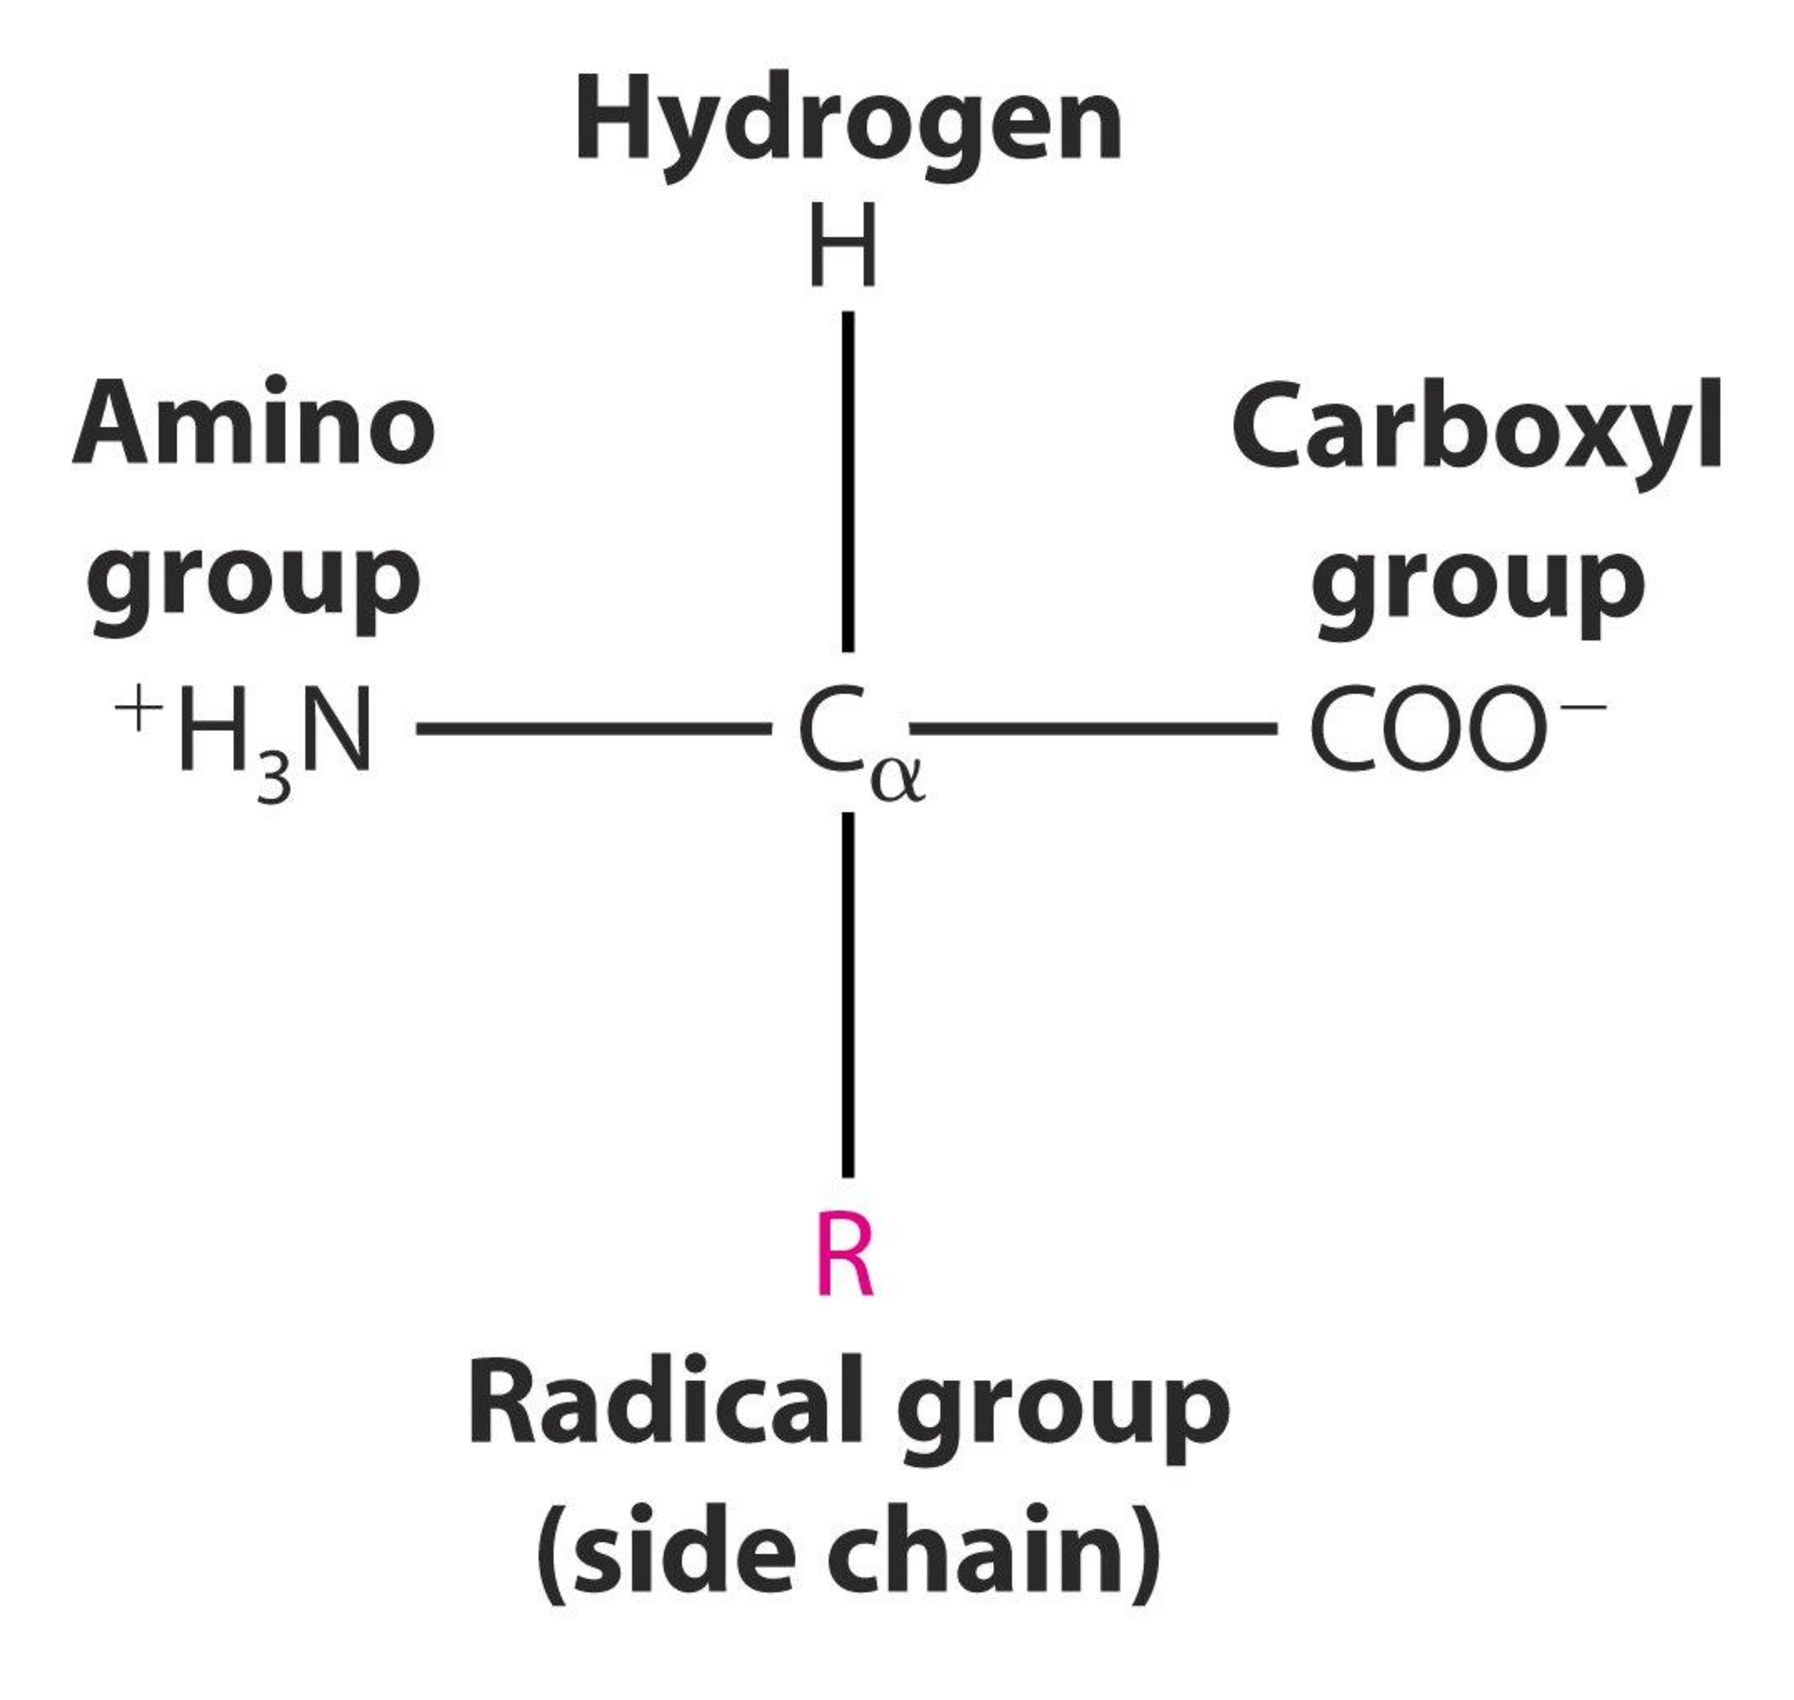
\includegraphics[width=0.35\textwidth]{graphics/amino_acid_structure.eps}
  \caption{Amino acid structure}
  \label{fig:amino_acid_structure}
\end{figure}
\FloatBarrier

Protein is constructed when multiple amino acids are combined into a string by a
peptide bond between the carboxyl group of one acid and the amino group of
another (giving $\mathrm{H}_{2}\mathrm{O}$ as a by-product).

\begin{figure}[h!]
  \centering
  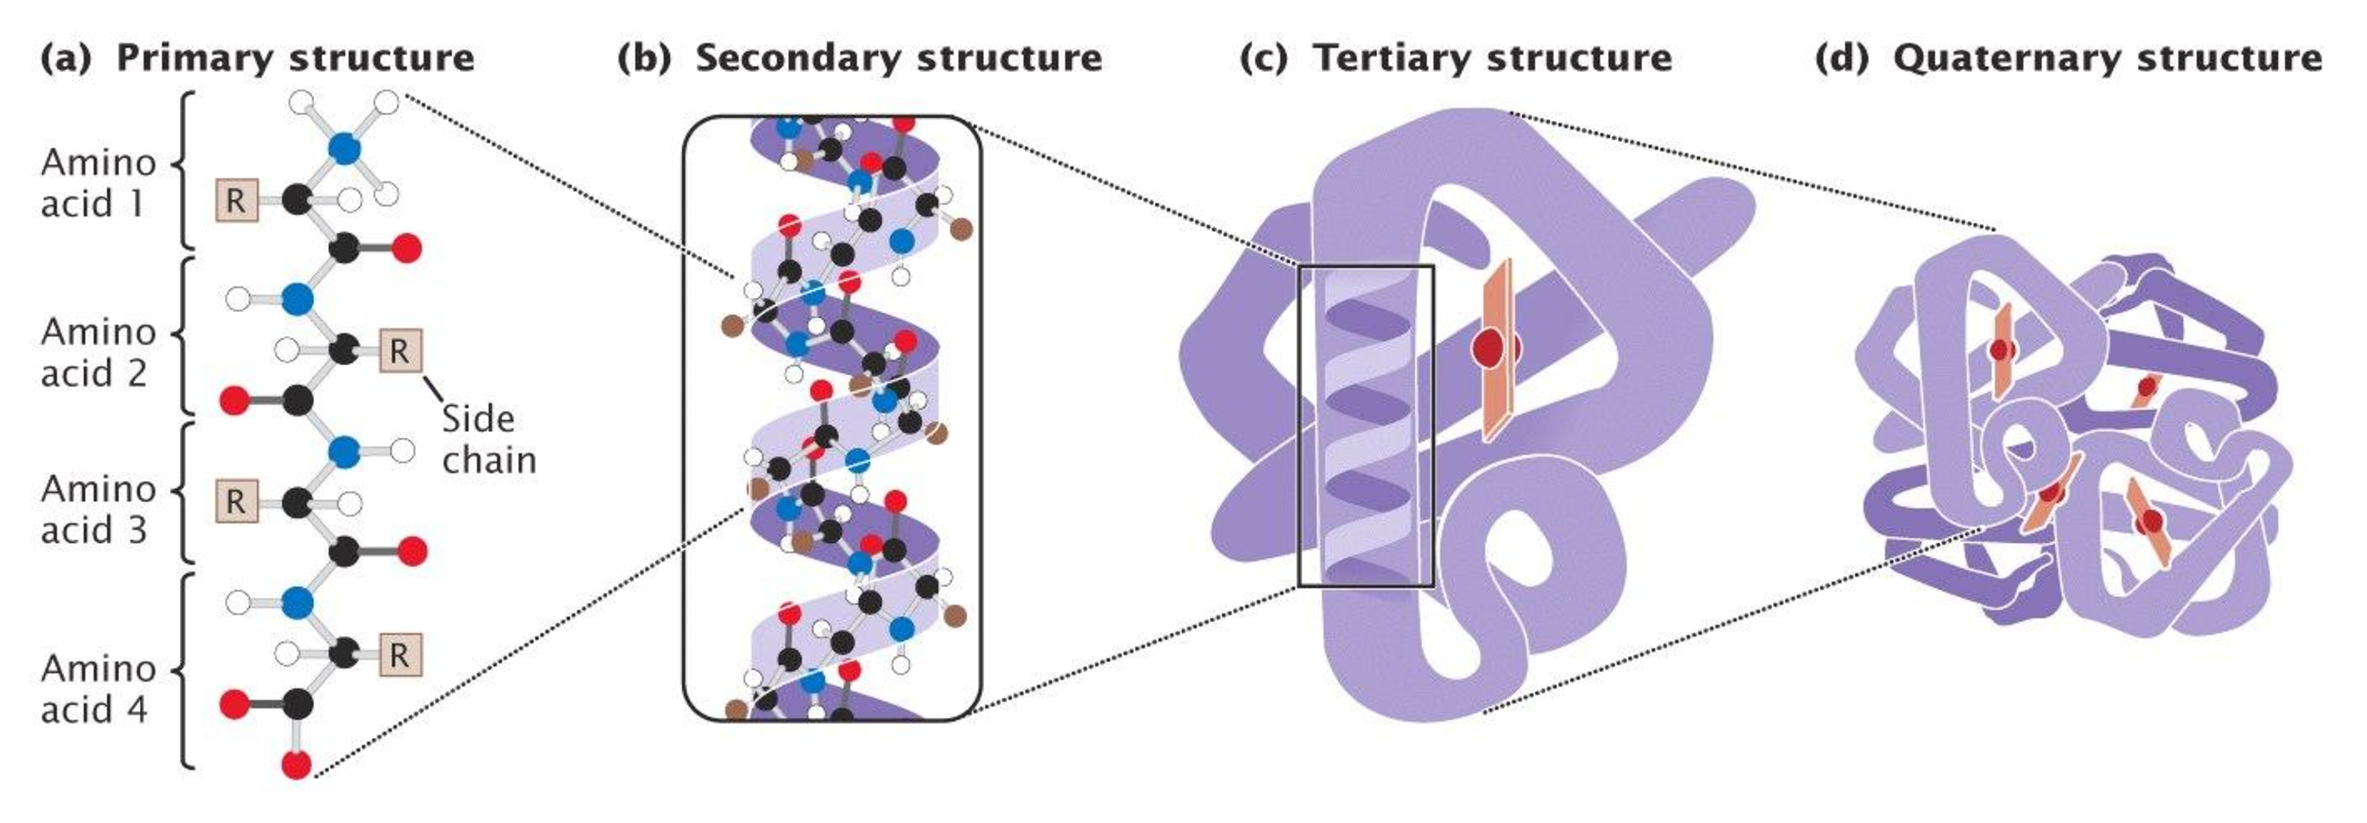
\includegraphics[width=\textwidth]{graphics/protein_structure.eps}
  \caption{Protein structure}
  \label{fig:protein_structure}
\end{figure}
\FloatBarrier

\subsubsection{Ribosomes}

\begin{itemize}
  \item Bind to the region of the mRNA that lies just upstream of the AUG codon
  \item Ribosome Binding Site (RBS) given a consensus sequence which varies with
        organism
\end{itemize}

\subsubsection{Translation process}

\begin{enumerate}
  \item[0] Binding of amino acid to tRNA
  \item[1] Initiation
    \begin{itemize}
      \item Ribosome recognition
        \begin{itemize}
          \item Prokaryotes: mRNA RBS hydrogen bonds with rRNA
          \item Eukaryotes: ribosome attaches to $5^{\prime}$ cap
        \end{itemize}
      \item $\mathrm{tRNA}^{\mathrm{met}}$ binds to AUG codon
    \end{itemize}
  \item[2] Elongation
  \item[3] Termination
    \begin{itemize}
      \item Ribosome pauses at stop codon
      \item Release factor binds
    \end{itemize}
\end{enumerate}

\subsubsection{Control of Gene Expression}

\begin{itemize}
  \item Various levels of control:
    \begin{itemize}
      \item Transcription
      \item Post-transcription
      \item Translation
      \item Post-translation
    \end{itemize}
\end{itemize}

\section{Genome Sequencing, Assembly and Annotation}

\subsection{Sequencing}

Reasons for sequencing:

\begin{itemize}
  \item Identify content and structure
  \item Identify mutations
\end{itemize}

The process of sequencing produces reads. A read is a single continuous sequence
read by the sequencing process.

\subsubsection{Sanger sequencing}

\begin{itemize}
  \item
    Uses DNA polymerase to synthesise DNA

    Enzyme that when given a DNA strand will synthesise the complementary strand

  \item
    A mixture of the polymerase, a primer (small strand of complimentary DNA)
    and deoxynucleotides (DNA nucleotides with fluorescent tag) is made.

  \item
    Products then separated. Multiple methods exist but traditionally using gel
    electrophoresis which allows florescent markers to be seen in four distinct
    "lanes" corresponding to each DNA nucleotide.

  \item
    Accurate but slow

\end{itemize}

\subsubsection{454 pyro-sequencing}

\begin{itemize}
  \item High throughput and lower sample preparation time
\end{itemize}

\subsubsection{Illumina Solexa approach}

\begin{itemize}
  \item Sequencing based on synthesis
  \item Lower cost per sequenced base but high initial cost
\end{itemize}

\subsubsection{Nanopore}

\begin{itemize}
  \item
    Feed DNA through a pore in a surface and detect nucleotides as they pass
    through

  \item
    Faster with minimal sample preparation

\end{itemize}

\subsection{Assembly}

Sequencing produces several fragments of the full genome, in order to obtain the
sequence of the full genome such subsequences must be assembled.

Individual reads are assembled to form contigs. A contig is a group of copied
pieces of DNA representing overlapping regions of a chromosome.

Contigs are assembled to give complete sequences.

\subsubsection{Shotgun sequencing}

\begin{itemize}
  \item
    Long sequences are assembled based on overlaps between several subsequences

  \item
    Region in full sequence should ideally be covered by several subsequences
    to ensure good confidence

    For Sanger sequencing 6 fold redundancy is required

  \item
    Nucleotide at a given position in the final sequence is given by the most
    common nucleotide in the aligned reads/contigs

  \item
    Assembly can be parameterised in terms of number of mismatches between
    aligned reads/contigs allowed at a given point in the final sequence

  \item
    Computationally intensive method: uses naive string searching which becomes
    very slow for large genomes and large number of reads

\end{itemize}

\subsubsection{deBruijn assembly}

\begin{itemize}
  \item
    Split data into a series of small equal length oliomers where oliomers are
    generated by advancing a sliding window along a sequence one nucleotide at a
    time

  \item
    Build a deBruijn graph of all oliomers where edges represent an alignment
    between the two joined oliomers

  \item
    If successful the graph structure will be a single string containing the
    aligned sequence, where the sequence forms an Euclidean path through all
    nodes

  \item
    The choice of the length $k$ of the oliomers is critical to the algorithm
    operating correctly.

    A sub-optimal value of $k$ will cause closed loops in the graph which
    prevents the correct sequence being obtained

\end{itemize}

\subsubsection{Finishing}

After alignment several gaps may be left in the final sequence, leaving the
result as a series of contigs.

Can be caused by lack of experimental data or issues with the wet experiment,
i.e. AT/GC right regions, homopolymenrs, etc.

Ideal solution is to perform more wet experiments.

\subsubsection{Templates}

When assembling the sequence of a new organism with known relatives the genomic
sequence of the relative can be used to assist positioning of the individual
contigs.

This is done by aligning the contigs to the genomic sequence of the relative.

\subsection{Annotation}

Consensus sequences are analysed to discover features details of which are
stored along with the sequence and the region of the sequence it is relevant to.

Typically a time and resource intensive task in the form of a pipeline of
individual tools used to identify specific features.

\subsubsection{Gene finding}

Open reading frames are a region starting with the initialisation codon
(\texttt{ATG}) and ending in one of three stop codons.

Gene finding can be done using one of two main approaches; comparative genomics
or ab initio.

Comparative genomics uses similarity between regions in a sample and other known
samples to infer the structure of a gene.

Ab initio methods are based on determining gene structure based solely on the
experimental data and known biological theories. External data can be used to
improve prediction accuracy.

Prediction of protein coding genes in bacterial genomes is simple and relatively
accurate. In eukaryotes predicting intron-exon regions is only around 65\%
accurate and non-coding exons can cause issues.

\section{Evolution}

Key relevance is similarity between close evolutionary ancestors which aids
prediction of features such as protein function and structure from a sequence.

\subsection{Mutations}

\Para{Point Mutation}

When a single nucleotide in the DNA sequence changes.

This can have several different effects on the protein sequence:

\begin{description}
  \item[Silent] \hfill \\
    The change in DNA sequence does not change the protein sequence.

    e.g. the mutation \texttt{TTC $\rightarrow$ TTT} gives
    \texttt{Lys $\rightarrow$ Lys}

  \item[Nonsense] \hfill \\
    The change in DNA sequence causes a change in protein sequence that does not
    make sense.

    e.g. the mutation \texttt{TTC $\rightarrow$ ATC} gives
    \texttt{Lys $\rightarrow$ STOP}

  \item[Missense] \hfill \\
    The change in DNA sequence causes a change in protein sequence that is valid
    but may affect the function.

    This can be either conservative in which case the new protein has a similar
    function to the previous or non-conservative in which case the functional
    change is significant.

\end{description}

\Para{Deletion}

Where a section of the sequence is removed.

\Para{Duplication}

Where a section of the sequence is duplicated and inserted after the original
section.

\Para{Inversion}

Where a section of the sequence is reversed in the new sequence.

\Para{Insertion}

Where a section of the sequence of one chromosome is inserted into the sequence
of another chromosome.

\Para{Translocation}

Where two sections of the sequence of two different chromosomes are swapped.

\Para{Frameshift mutations}

Mutations where the relative location of coding information is changed due to
the insertion, deletion or exchange of a subsequence of a different length to
the original.

\subsubsection{Gene duplication}

\begin{itemize}
  \item
    Evolutionary constraints define the tolerance of how much the gene can
    diverge from its original function after an evolutionary cycle.

  \item
    After gene duplication duplicates have reduced evolutionary constraints as
    the original copy still exists therefore retention of the original function
    is less important.

  \item
    Gene duplication leads to wider divergence in function and evolution of new
    proteins.

  \item
    In bacteria gene duplication can be triggered by external stimuli.

    e.g. temperature, pressure, starvation, etc.

  \item
    In eukaryotes gene duplication is vital for evolution. Around $\frac{1}{3}$
    of a eukaryotic genome consists of duplicates.

  \item
    Duplicate genes with redundant functions can help towards protection against
    deletion mutations.

\end{itemize}

\subsection{Homology, orthology and parology}

\begin{description}
  \item[Homology] \hfill \\
    Genes that share a common ancestor.

  \item[Orthology] \hfill \\
    Homologous genes which diverged as a result of speciation.

  \item[Parology] \hfill \\
    Homologous genes within the same genome created as a result of gene
    duplication.

  \item[Xenology] \hfill \\
    Homologous genes where one gene has been obtained through transfer of
    genetic material between organisms.

\end{description}

\begin{figure}[h!]
  \centering
  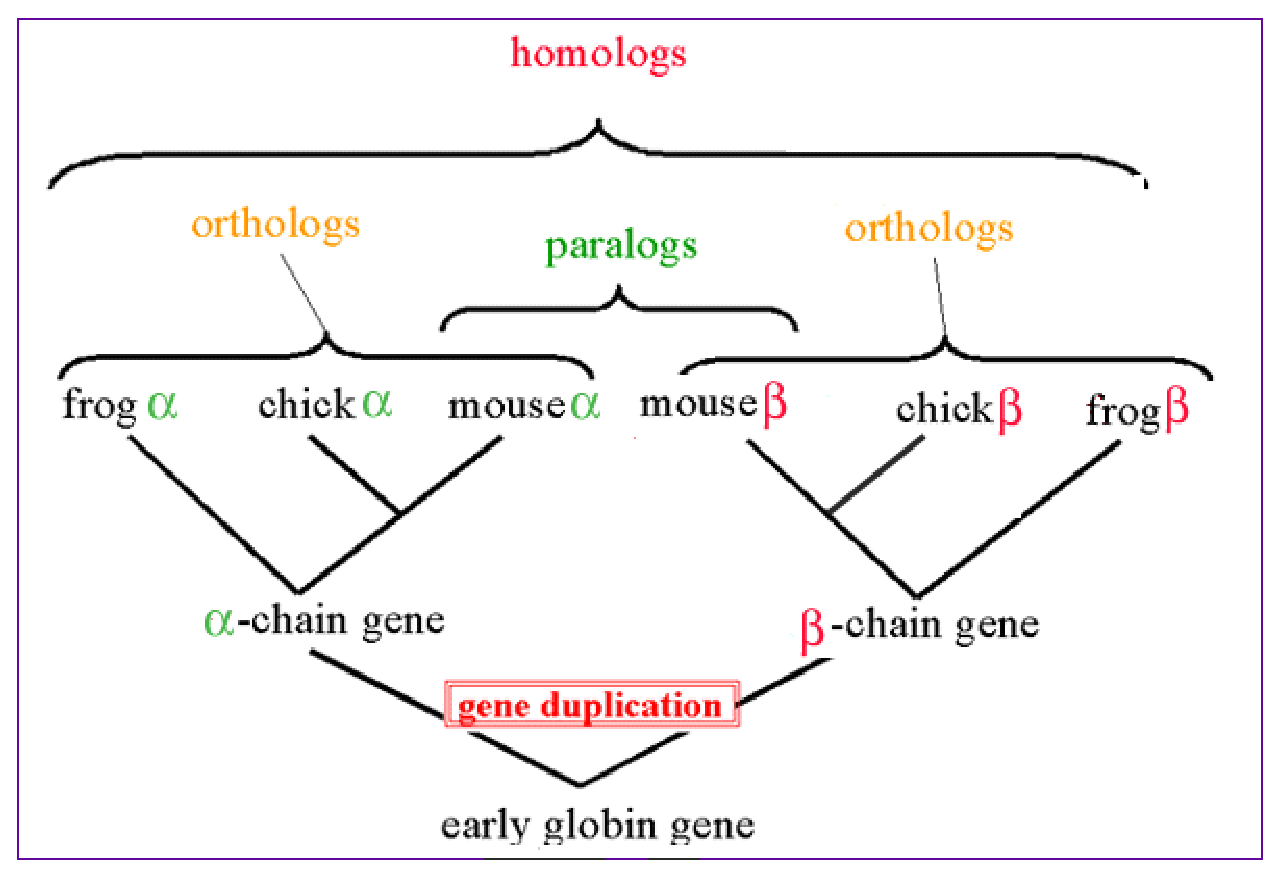
\includegraphics[width=0.7\textwidth]{graphics/homology_orthology_parology.eps}
  \caption{Relationship between homology, orthology and parology}
  \label{fig:homology_orthology_parology}
\end{figure}
\FloatBarrier

\subsection{Homology}

\begin{itemize}
  \item
    Proteins and genes that have diverged from a common ancestor are homologous.

  \item
    Homology is a boolean state, not analogous to sequence similarity.

  \item
    Homology cannot be definitively determined from sequence similarity alone,
    it can however be inferred if the sequences are more than 50\% similar.

  \item
    Homologous proteins often share properties: same/related function, sites,
    structure.

  \item
    As sequences diverge non-conservative mutations increase and the sequence
    similarity to the common ancestor decreases while remaining functionally
    similar, this can make determining homology difficult.

\end{itemize}

\subsection{Orthology}

\begin{itemize}
  \item
    Homologous genes from different genomes within the same gene family.

  \item
    Derived as a result of speciation.

  \item
    Often encode proteins that perform the same function in different organisms.

\end{itemize}

\subsection{Parology}

\begin{itemize}
  \item
    Homologous genes within the same genome within different gene families.

  \item
    May perform different functions in each host due to functional change with
    evolution.
\end{itemize}

\section{Phylogenetics}

\begin{itemize}
  \item
    The study of evolutionary relationships between groups of organisms.

  \item
    Produces hypothesis about evolutionary history of organisms.

  \item
    Species (genes) typically shows as evolving as per a tree structure.

  \item
    Based on inferring information about evolutionary history from present day
    knowledge.

    Phylogenetics are hypotheses.

    Changes as new data becomes available.

  \item
    Can use molecular data to infer phylogenetic relationships.
\end{itemize}

\subsection{Workflow}

\subsubsection{Obtain sequences}

\begin{itemize}
  \item
    Selection of sequences is dependant on the research.

  \item
    Typically use well conserved genes.
\end{itemize}

\subsubsection{Alignment}

\begin{itemize}
  \item
    TODO
\end{itemize}

\subsubsection{Masking}

\begin{itemize}
  \item
    Separate areas of high similarity from those of low similarity.

  \item
    Areas of high similarity infer homology, low similarity cannot be used to
    infer either way.

\end{itemize}

\subsubsection{Evolutionary model fitting}

\begin{itemize}
  \item
    TODO
\end{itemize}

\subsubsection{Analyse tree}

\begin{itemize}
  \item
    Tips correspond to modern species.

  \item
    Position of fork in tree in terms of depth is reflective of the point in
    history that the two organisms diverged.

\end{itemize}

\section{Sequence Similarity and Comparison}

TODO

\section{Protein Structure Prediction}

TODO

\section{Network Analysis}

TODO

\section{Omics Data ans Analysis}

TODO

\section{Data Standards}

TODO

\end{document}
